Alternatively to the approach described above, the
open-source workload managing system \Slurm~\cite{Slurm} has been interfaced into \Roced by
the ATLAS group at University of Freiburg.
While \Slurm provides a built-in functionality for dynamic
startup of resources in the \textit{Slurm Elastic Computing} module~\cite{SlurmElastic}, this has been found to be unsuitable for resources which are not
expected to be available within a fixed time period, in this case due to
the presence of a queue in the host system which may postpone the start
of a resource by a significant, varying period.
In addition the transfer of information, such as error states, from one scheduler to the
other, and therefore to the user, is very limited.
Therefore, \Roced has been chosen as the interface between the
\Moab scheduler on the host system and the \Slurm
scheduler on the submission side.


\begin{figure}

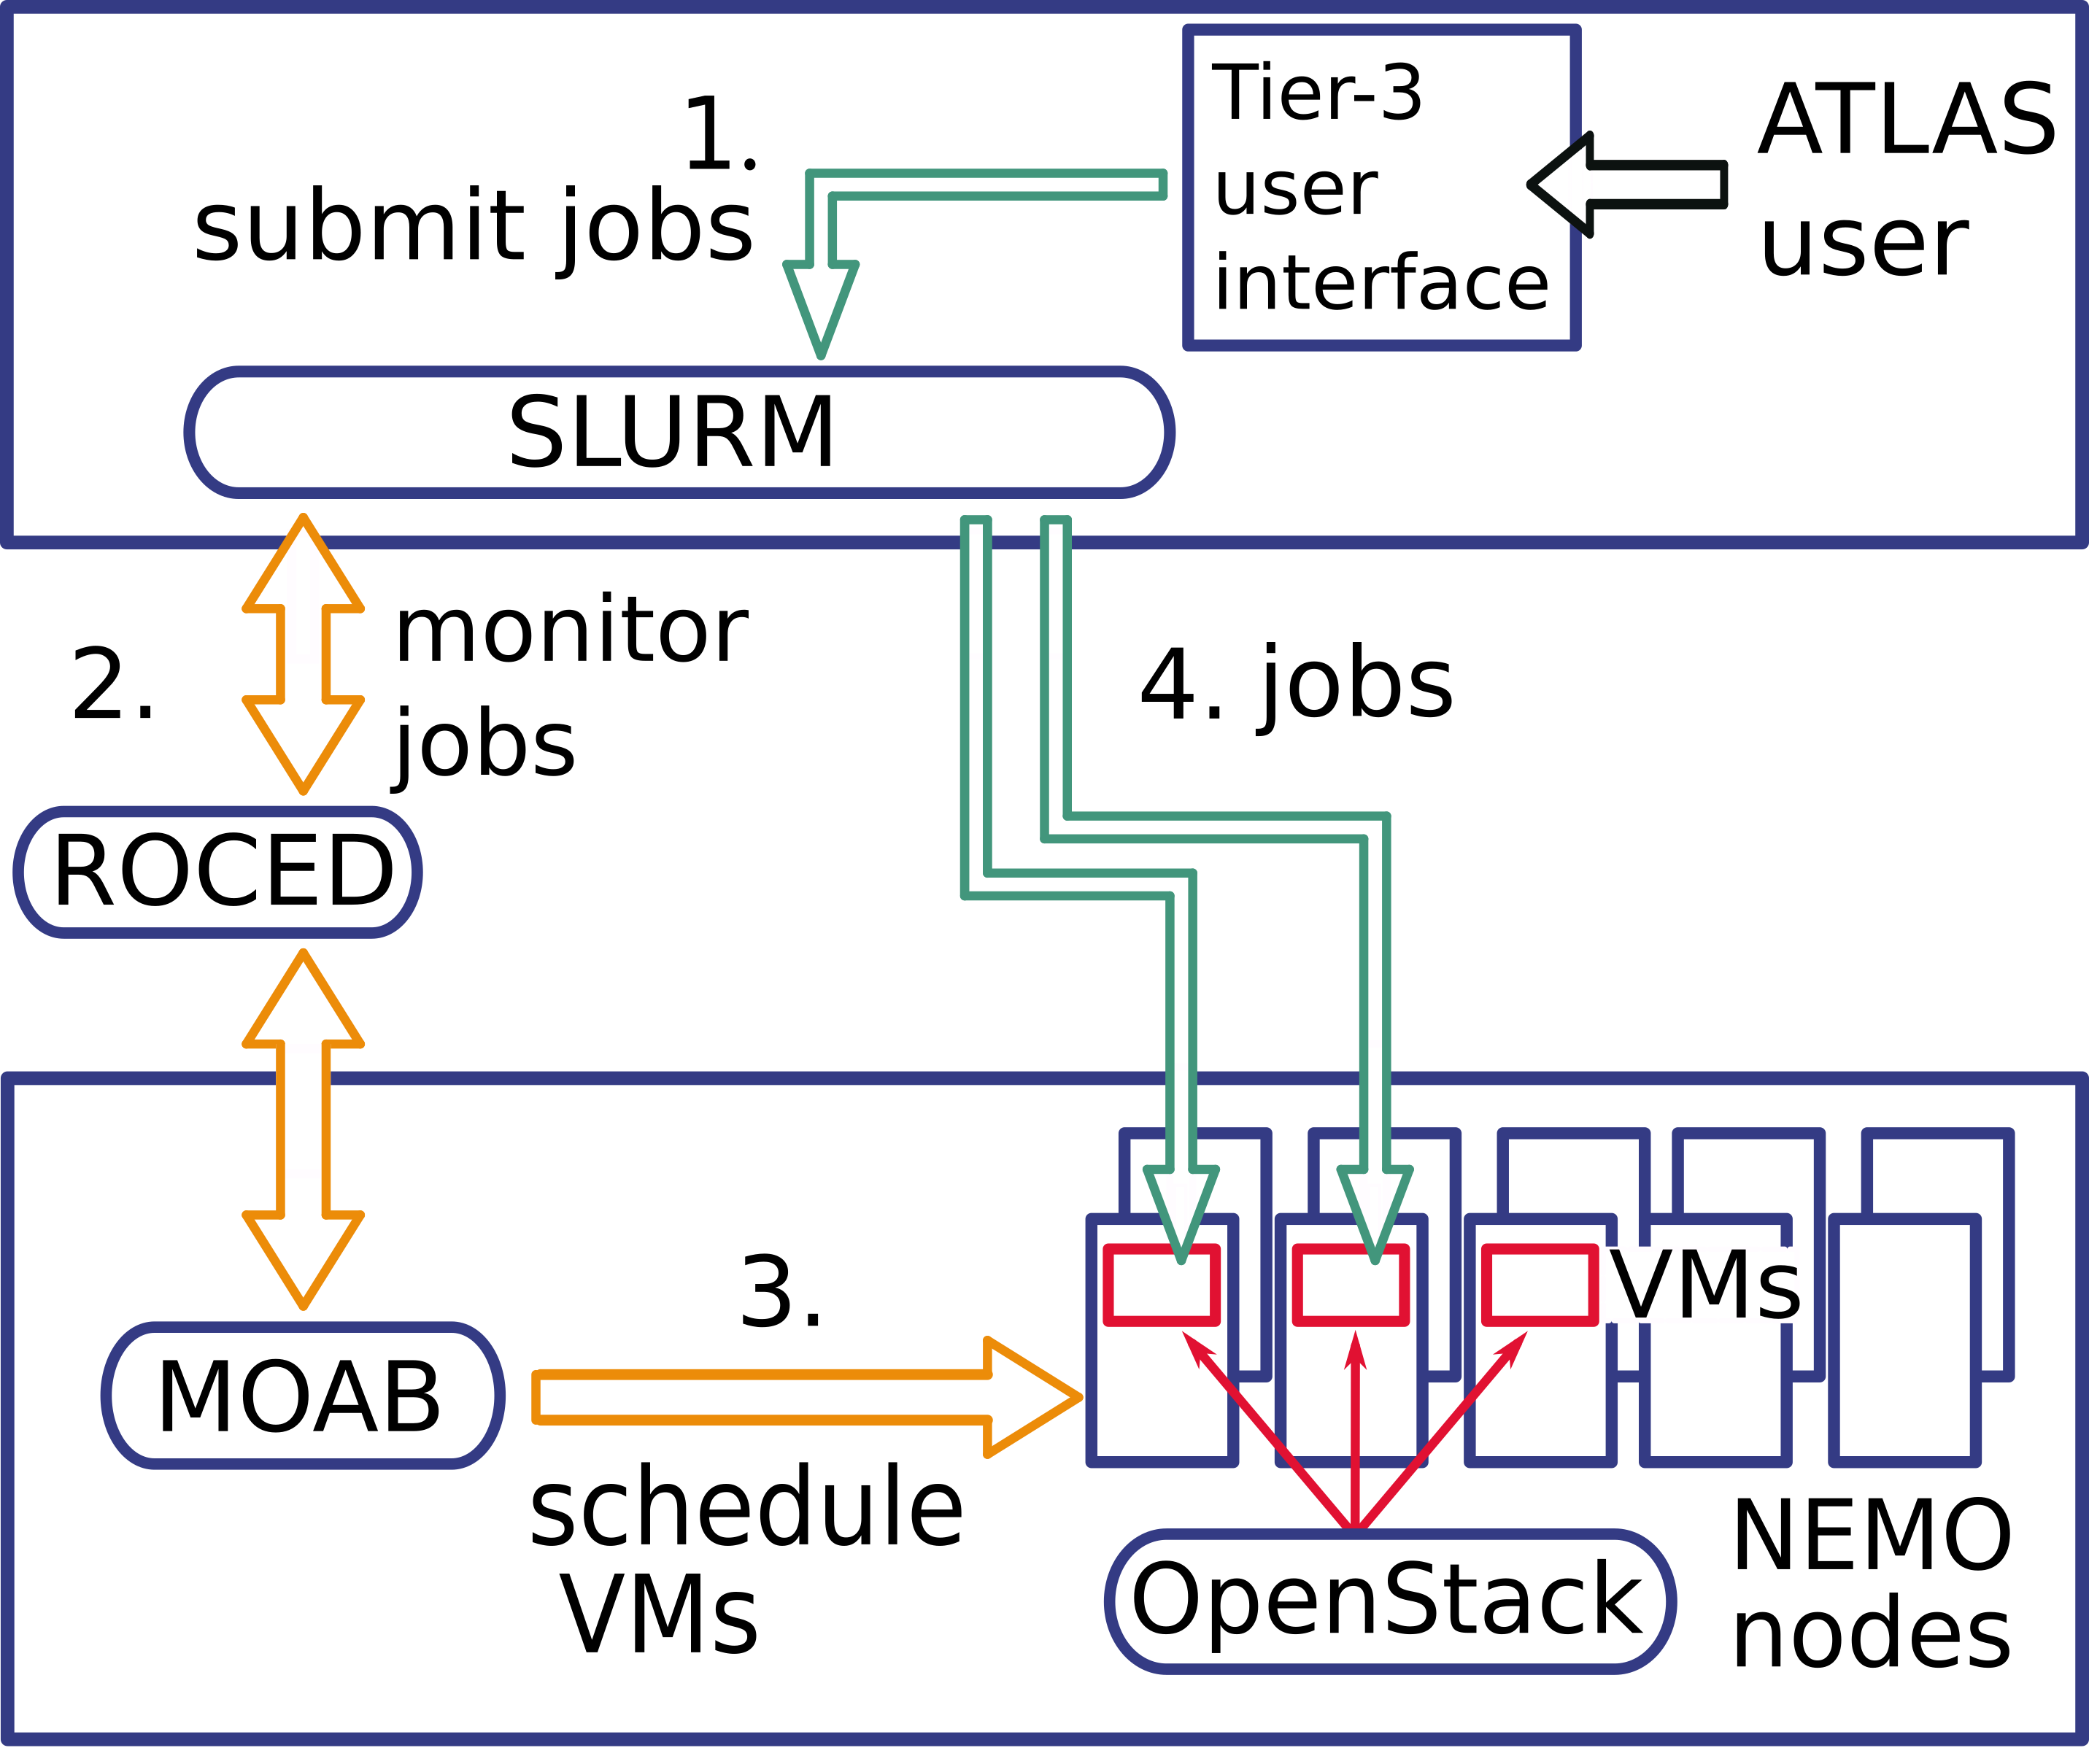
\includegraphics[width=0.95\linewidth]{figures/virtualisierung_ROCED.png}
\caption{Implementation of \Roced with \Slurm on the BFG cluster used by ATLAS researchers.}
\label{fig:slurmRocedBFG}
\end{figure}

The scheduling system is illustrated in Fig.~\ref{fig:slurmRocedBFG}.
For \Slurm, it is necessary that each potential virtual
machine is registered in the configuration at the time of start of the
\Slurm server as well as the client. \Slurm configurations also
need to be in agreement between server and client.
Therefore, a range of hostnames is registered in the configuration in
a way that is mapped to potential IP addresses of virtual machines.
These virtual machines have a fixed number of CPUs and memory assigned and are
registered under a certain \Slurm partition.
When a job is submitted to this partition and no other resource is
available, information from the \Slurm \texttt{squeue} and
\texttt{sinfo} commands is requested and parsed for the required information.

Since the ATLAS Freiburg group comprises three sub-groups, each mapped
to a different production account on \NEMO, special care is taken to
avoid interference of resources used by another account to ensure fair share on \NEMO, while
allowing jobs from one group to occupy otherwise idle resources of another group.

\Roced determines the amount of virtual machines to be started and sends the
corresponding VRE job submission commands to \Moab.
After the virtual machine has booted, the hostname is set to the IP
dependent name which is known to the \Slurm configuration.
A \texttt{cron} job executes several sanity
checks on the system.
Upon successful execution of these tests, the \Slurm client
running in the VM starts accepting the queued jobs.
After completion of the jobs and a certain period of receiving no new jobs from the queue, the
\Slurm client in the machine drains itself and the machine
shuts itself down.
The IP address as well as the corresponding hostname in \Slurm
are released and can be reused by future VREs.
